\documentclass{ximera}

%\usepackage{todonotes}

\newcommand{\todo}{}

\usepackage{esint} % for \oiint
\ifxake%%https://math.meta.stackexchange.com/questions/9973/how-do-you-render-a-closed-surface-double-integral
\renewcommand{\oiint}{{\large\bigcirc}\kern-1.56em\iint}
\fi


\graphicspath{
  {./}
  {ximeraTutorial/}
  {basicPhilosophy/}
  {functionsOfSeveralVariables/}
  {normalVectors/}
  {lagrangeMultipliers/}
  {vectorFields/}
  {greensTheorem/}
  {shapeOfThingsToCome/}
  {dotProducts/}
  {partialDerivativesAndTheGradientVector/}
  {../productAndQuotientRules/exercises/}
  {../normalVectors/exercisesParametricPlots/}
  {../continuityOfFunctionsOfSeveralVariables/exercises/}
  {../partialDerivativesAndTheGradientVector/exercises/}
  {../directionalDerivativeAndChainRule/exercises/}
  {../commonCoordinates/exercisesCylindricalCoordinates/}
  {../commonCoordinates/exercisesSphericalCoordinates/}
  {../greensTheorem/exercisesCurlAndLineIntegrals/}
  {../greensTheorem/exercisesDivergenceAndLineIntegrals/}
  {../shapeOfThingsToCome/exercisesDivergenceTheorem/}
  {../greensTheorem/}
  {../shapeOfThingsToCome/}
  {../separableDifferentialEquations/exercises/}
  {vectorFields/}
}

\newcommand{\mooculus}{\textsf{\textbf{MOOC}\textnormal{\textsf{ULUS}}}}

\usepackage{tkz-euclide}
\usepackage{tikz}
\usepackage{tikz-cd}
\usetikzlibrary{arrows}
\tikzset{>=stealth,commutative diagrams/.cd,
  arrow style=tikz,diagrams={>=stealth}} %% cool arrow head
\tikzset{shorten <>/.style={ shorten >=#1, shorten <=#1 } } %% allows shorter vectors

\usetikzlibrary{backgrounds} %% for boxes around graphs
\usetikzlibrary{shapes,positioning}  %% Clouds and stars
\usetikzlibrary{matrix} %% for matrix
\usepgfplotslibrary{polar} %% for polar plots
\usepgfplotslibrary{fillbetween} %% to shade area between curves in TikZ
%\usetkzobj{all}
\usepackage[makeroom]{cancel} %% for strike outs
%\usepackage{mathtools} %% for pretty underbrace % Breaks Ximera
%\usepackage{multicol}
\usepackage{pgffor} %% required for integral for loops



%% http://tex.stackexchange.com/questions/66490/drawing-a-tikz-arc-specifying-the-center
%% Draws beach ball
\tikzset{pics/carc/.style args={#1:#2:#3}{code={\draw[pic actions] (#1:#3) arc(#1:#2:#3);}}}



\usepackage{array}
\setlength{\extrarowheight}{+.1cm}
\newdimen\digitwidth
\settowidth\digitwidth{9}
\def\divrule#1#2{
\noalign{\moveright#1\digitwidth
\vbox{\hrule width#2\digitwidth}}}




% \newcommand{\RR}{\mathbb R}
% \newcommand{\R}{\mathbb R}
% \newcommand{\N}{\mathbb N}
% \newcommand{\Z}{\mathbb Z}

\newcommand{\sagemath}{\textsf{SageMath}}


%\renewcommand{\d}{\,d\!}
%\renewcommand{\d}{\mathop{}\!d}
%\newcommand{\dd}[2][]{\frac{\d #1}{\d #2}}
%\newcommand{\pp}[2][]{\frac{\partial #1}{\partial #2}}
% \renewcommand{\l}{\ell}
%\newcommand{\ddx}{\frac{d}{\d x}}

% \newcommand{\zeroOverZero}{\ensuremath{\boldsymbol{\tfrac{0}{0}}}}
%\newcommand{\inftyOverInfty}{\ensuremath{\boldsymbol{\tfrac{\infty}{\infty}}}}
%\newcommand{\zeroOverInfty}{\ensuremath{\boldsymbol{\tfrac{0}{\infty}}}}
%\newcommand{\zeroTimesInfty}{\ensuremath{\small\boldsymbol{0\cdot \infty}}}
%\newcommand{\inftyMinusInfty}{\ensuremath{\small\boldsymbol{\infty - \infty}}}
%\newcommand{\oneToInfty}{\ensuremath{\boldsymbol{1^\infty}}}
%\newcommand{\zeroToZero}{\ensuremath{\boldsymbol{0^0}}}
%\newcommand{\inftyToZero}{\ensuremath{\boldsymbol{\infty^0}}}



% \newcommand{\numOverZero}{\ensuremath{\boldsymbol{\tfrac{\#}{0}}}}
% \newcommand{\dfn}{\textbf}
% \newcommand{\unit}{\,\mathrm}
% \newcommand{\unit}{\mathop{}\!\mathrm}
% \newcommand{\eval}[1]{\bigg[ #1 \bigg]}
% \newcommand{\seq}[1]{\left( #1 \right)}
% \renewcommand{\epsilon}{\varepsilon}
% \renewcommand{\phi}{\varphi}


% \renewcommand{\iff}{\Leftrightarrow}

% \DeclareMathOperator{\arccot}{arccot}
% \DeclareMathOperator{\arcsec}{arcsec}
% \DeclareMathOperator{\arccsc}{arccsc}
% \DeclareMathOperator{\si}{Si}
% \DeclareMathOperator{\scal}{scal}
% \DeclareMathOperator{\sign}{sign}


%% \newcommand{\tightoverset}[2]{% for arrow vec
%%   \mathop{#2}\limits^{\vbox to -.5ex{\kern-0.75ex\hbox{$#1$}\vss}}}
% \newcommand{\arrowvec}[1]{{\overset{\rightharpoonup}{#1}}}
% \renewcommand{\vec}[1]{\arrowvec{\mathbf{#1}}}
% \renewcommand{\vec}[1]{{\overset{\boldsymbol{\rightharpoonup}}{\mathbf{#1}}}}

% \newcommand{\point}[1]{\left(#1\right)} %this allows \vector{ to be changed to \vector{ with a quick find and replace
% \newcommand{\pt}[1]{\mathbf{#1}} %this allows \vec{ to be changed to \vec{ with a quick find and replace
% \newcommand{\Lim}[2]{\lim_{\point{#1} \to \point{#2}}} %Bart, I changed this to point since I want to use it.  It runs through both of the exercise and exerciseE files in limits section, which is why it was in each document to start with.

% \DeclareMathOperator{\proj}{\mathbf{proj}}
% \newcommand{\veci}{{\boldsymbol{\hat{\imath}}}}
% \newcommand{\vecj}{{\boldsymbol{\hat{\jmath}}}}
% \newcommand{\veck}{{\boldsymbol{\hat{k}}}}
% \newcommand{\vecl}{\vec{\boldsymbol{\l}}}
% \newcommand{\uvec}[1]{\mathbf{\hat{#1}}}
% \newcommand{\utan}{\mathbf{\hat{t}}}
% \newcommand{\unormal}{\mathbf{\hat{n}}}
% \newcommand{\ubinormal}{\mathbf{\hat{b}}}

% \newcommand{\dotp}{\bullet}
% \newcommand{\cross}{\boldsymbol\times}
% \newcommand{\grad}{\boldsymbol\nabla}
% \newcommand{\divergence}{\grad\dotp}
% \newcommand{\curl}{\grad\cross}
%\DeclareMathOperator{\divergence}{divergence}
%\DeclareMathOperator{\curl}[1]{\grad\cross #1}
% \newcommand{\lto}{\mathop{\longrightarrow\,}\limits}

% \renewcommand{\bar}{\overline}

\colorlet{textColor}{black}
\colorlet{background}{white}
\colorlet{penColor}{blue!50!black} % Color of a curve in a plot
\colorlet{penColor2}{red!50!black}% Color of a curve in a plot
\colorlet{penColor3}{red!50!blue} % Color of a curve in a plot
\colorlet{penColor4}{green!50!black} % Color of a curve in a plot
\colorlet{penColor5}{orange!80!black} % Color of a curve in a plot
\colorlet{penColor6}{yellow!70!black} % Color of a curve in a plot
\colorlet{fill1}{penColor!20} % Color of fill in a plot
\colorlet{fill2}{penColor2!20} % Color of fill in a plot
\colorlet{fillp}{fill1} % Color of positive area
\colorlet{filln}{penColor2!20} % Color of negative area
\colorlet{fill3}{penColor3!20} % Fill
\colorlet{fill4}{penColor4!20} % Fill
\colorlet{fill5}{penColor5!20} % Fill
\colorlet{gridColor}{gray!50} % Color of grid in a plot

\newcommand{\surfaceColor}{violet}
\newcommand{\surfaceColorTwo}{redyellow}
\newcommand{\sliceColor}{greenyellow}




\pgfmathdeclarefunction{gauss}{2}{% gives gaussian
  \pgfmathparse{1/(#2*sqrt(2*pi))*exp(-((x-#1)^2)/(2*#2^2))}%
}


%%%%%%%%%%%%%
%% Vectors
%%%%%%%%%%%%%

%% Simple horiz vectors
\renewcommand{\vector}[1]{\left\langle #1\right\rangle}


%% %% Complex Horiz Vectors with angle brackets
%% \makeatletter
%% \renewcommand{\vector}[2][ , ]{\left\langle%
%%   \def\nextitem{\def\nextitem{#1}}%
%%   \@for \el:=#2\do{\nextitem\el}\right\rangle%
%% }
%% \makeatother

%% %% Vertical Vectors
%% \def\vector#1{\begin{bmatrix}\vecListA#1,,\end{bmatrix}}
%% \def\vecListA#1,{\if,#1,\else #1\cr \expandafter \vecListA \fi}

%%%%%%%%%%%%%
%% End of vectors
%%%%%%%%%%%%%

%\newcommand{\fullwidth}{}
%\newcommand{\normalwidth}{}



%% makes a snazzy t-chart for evaluating functions
%\newenvironment{tchart}{\rowcolors{2}{}{background!90!textColor}\array}{\endarray}

%%This is to help with formatting on future title pages.
\newenvironment{sectionOutcomes}{}{}



%% Flowchart stuff
%\tikzstyle{startstop} = [rectangle, rounded corners, minimum width=3cm, minimum height=1cm,text centered, draw=black]
%\tikzstyle{question} = [rectangle, minimum width=3cm, minimum height=1cm, text centered, draw=black]
%\tikzstyle{decision} = [trapezium, trapezium left angle=70, trapezium right angle=110, minimum width=3cm, minimum height=1cm, text centered, draw=black]
%\tikzstyle{question} = [rectangle, rounded corners, minimum width=3cm, minimum height=1cm,text centered, draw=black]
%\tikzstyle{process} = [rectangle, minimum width=3cm, minimum height=1cm, text centered, draw=black]
%\tikzstyle{decision} = [trapezium, trapezium left angle=70, trapezium right angle=110, minimum width=3cm, minimum height=1cm, text centered, draw=black]


\title{Accumulation}

\begin{document}

\begin{abstract}
adding rates
\end{abstract}
\maketitle





Suppose you are driving a car at a constant velocity (rate of change) of 20 miles per hour. 20 miles per hour tells us how the miles are changing compared to the change in hours.  Whenever the time \textbf{\textcolor{purple!85!blue}{changes}} by $1$ hour, the distance travelled \textbf{\textcolor{purple!85!blue}{changes}} by $20$ miles.

\[
\text{rate of change} = \text{velocity} = \text{20 miles per hour} = \frac{20 \, miles}{1 \, hour} = \frac{\Delta miles}{\Delta hours}
\]

\textbf{Note:} Our symbol for ``the change in'' is the uppercase Greek letter delta, $\Delta$. \\

The graph of velocity would be a horizontal line.



\begin{image}
\begin{tikzpicture}
  \begin{axis}[
            domain=0:10, ymax=100, xmax=10, ymin=0, xmin=0,
            axis lines =center, xlabel=$t$, ylabel=$v$, 
            ytick={0, 10, 20, 30, 40, 50, 60, 70, 80, 90},
            xtick={0, 2, 4, 6, 8, 10},
            ticklabel style={font=\scriptsize},
            every axis y label/.style={at=(current axis.above origin),anchor=south},
            every axis x label/.style={at=(current axis.right of origin),anchor=west},
            axis on top
          ]
          

			\addplot [draw=penColor, very thick, smooth, domain=(0:8),->] {20};
			\addplot[color=penColor,fill=penColor,only marks,mark=*] coordinates{(0,20)};



  \end{axis}
\end{tikzpicture}
\end{image}

In the velocity story, we know that the car's distance changes by 20 miles every time the time changes by 1 hour.  The reverse of this rate of change story is an accumulation story.

Suppose we let time run for a while, how far does the car travel?  How much distance is accumulated?



\subsection*{Accumulation}


To get the accumulated distance, we multiply the velocity by the time.

\[
Distance = Velocity \cdot Time = \frac{\Delta miles}{\Delta hours} \cdot \Delta hours = \Delta miles
\]


We can get a geometric interpretation of this in our velocity graph.




In that graph, miles per hour are the vertical units and hours are the horizontal units.  We can represent $\frac{\Delta miles}{\Delta hours} \cdot \Delta hours$ as the area of the rectangle underneath the graph of velocity.





\begin{image}
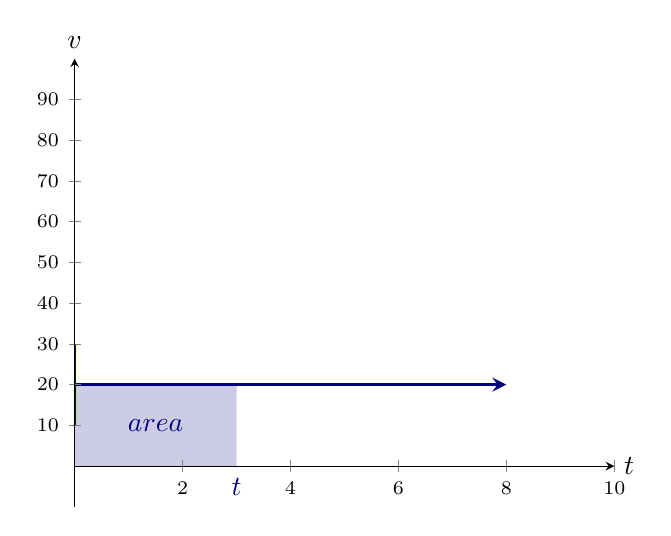
\begin{tikzpicture}
  \begin{axis}[
            domain=0:10, ymax=100, xmax=10, ymin=-10, xmin=0,
            axis lines =center, xlabel=$t$, ylabel=$v$, 
            ytick={0, 10, 20, 30, 40, 50, 60, 70, 80, 90},
            xtick={0, 2, 4, 6, 8, 10},
            ticklabel style={font=\scriptsize},
            every axis y label/.style={at=(current axis.above origin),anchor=south},
            every axis x label/.style={at=(current axis.right of origin),anchor=west},
            axis on top
          ]
          

			\addplot [draw=penColor, very thick, smooth, domain=(0:8),->] {20};
			%\addplot[color=penColor,fill=penColor,only marks,mark=*] coordinates{(0,50)};



			\addplot [name path=A,domain=0:3,draw=none] {20};   
			\addplot [name path=B,domain=0:3,draw=none] {0};
			\addplot [fillp] fill between[of=A and B];

			\draw[penColor,thick] (0,10) -- (0,30);
			\draw[penColor,thick] (30,10) -- (30,30);

			\node at (axis cs:1.5,10) [penColor] {$area$};
			\node at (axis cs:3,-5) [penColor] {$t$};



  \end{axis}
\end{tikzpicture}
\end{image}


\[
\text{Area } = \frac{\Delta \text{miles}}{\Delta \text{hours}} \cdot \Delta \text{hours} = \Delta \text{miles}
\]


The area under the graph of $v(t) = 20$ over the interval $(0, t)$ is given by $20 \, t$, which is a linear function.






The graph of accumulated distance, $D(t) = 20 \, t$ is a line with slope $20$.




\begin{image}
\begin{tikzpicture}
  \begin{axis}[
            domain=0:10, ymax=100, xmax=10, ymin=-10, xmin=0,
            axis lines =center, xlabel=$t$, ylabel=$D$, 
            ytick={0, 10, 20, 30, 40, 50, 60, 70, 80, 90},
            xtick={0, 2, 4, 6, 8, 10},
            ticklabel style={font=\scriptsize},
            every axis y label/.style={at=(current axis.above origin),anchor=south},
            every axis x label/.style={at=(current axis.right of origin),anchor=west},
            axis on top
          ]
          

			\addplot [draw=penColor, very thick, smooth, domain=(0:4),->] {20*x};
			%\addplot[color=penColor,fill=penColor,only marks,mark=*] coordinates{(0,50)};









  \end{axis}
\end{tikzpicture}
\end{image}
There is a reverse relationship between rate of change and accumulation. \\


$\blacktriangleright$ The value of $v(t)$ gives the rate of change of $D(t)$.


$\blacktriangleright$ The value of $D(t)$ gives the area under the graph of $v(t)$, between $0$ and $t$.






Of course, the constant function $v(t) = 20$ is also a linear function. Its rate of change is the constant function $0$.  We can view $v(t)$ as a function with a rate of change of $0$ or we can view it as the rate of change of some function, $D(t)$. This function, $D(t)$, is represented graphically by the area under the graph of $v(t)$.



$\blacktriangleright$  We can repeat this same story with $D(t)$.  \\


That is, we could view $D(t) = 20t$ as the rate of change of some function, $Q(t)$.  The function, $Q(t)$, would measure the area under the graph of $y = D(t)$.


What is the area under $y = D(t) = 20 \, t$?









\begin{image}
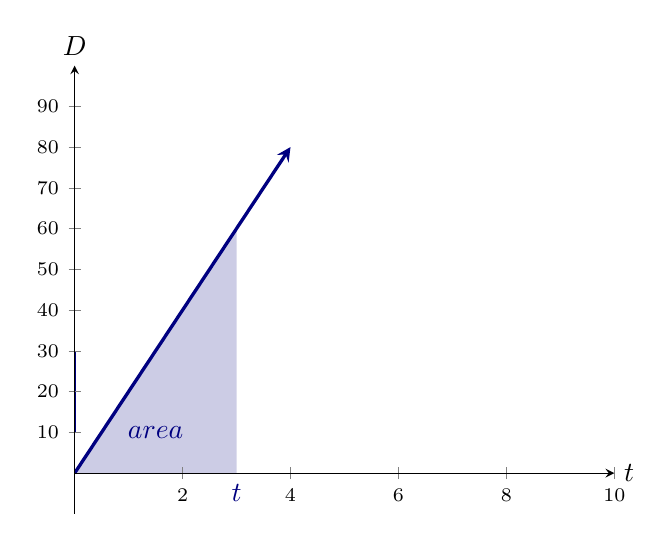
\begin{tikzpicture}
  \begin{axis}[
            domain=0:10, ymax=100, xmax=10, ymin=-10, xmin=0,
            axis lines =center, xlabel=$t$, ylabel=$D$, 
            ytick={0, 10, 20, 30, 40, 50, 60, 70, 80, 90},
            xtick={0, 2, 4, 6, 8, 10},
            ticklabel style={font=\scriptsize},
            every axis y label/.style={at=(current axis.above origin),anchor=south},
            every axis x label/.style={at=(current axis.right of origin),anchor=west},
            axis on top
          ]
          

			\addplot [draw=penColor, very thick, smooth, domain=(0:4),->] {20*x};
			%\addplot[color=penColor,fill=penColor,only marks,mark=*] coordinates{(0,50)};




			\addplot [name path=A,domain=0:3,draw=none] {20*x};   
			\addplot [name path=B,domain=0:3,draw=none] {0};
			\addplot [fillp] fill between[of=A and B];

			\draw[penColor,thick] (0,10) -- (0,30);
			\draw[penColor,thick] (30,10) -- (30,70);

			\node at (axis cs:1.5,10) [penColor] {$area$};
			\node at (axis cs:3,-5) [penColor] {$t$};




  \end{axis}
\end{tikzpicture}
\end{image}



Geometrically, we can see the region under the graph forms a triangle.


\begin{formula}
\[
Area(t) = \frac{1}{2} \, Base \cdot Height = \frac{1}{2}  \, \answer{t} \cdot \left(\answer{20 \, t}\right) = 10 \, t^2
\]
\end{formula}













\begin{image}
\begin{tikzpicture}
  \begin{axis}[
            domain=0:10, ymax=100, xmax=10, ymin=-10, xmin=0,
            axis lines =center, xlabel=$t$, ylabel=$A$, 
            ytick={0, 10, 20, 30, 40, 50, 60, 70, 80, 90},
            xtick={0, 2, 4, 6, 8, 10},
            ticklabel style={font=\scriptsize},
            every axis y label/.style={at=(current axis.above origin),anchor=south},
            every axis x label/.style={at=(current axis.right of origin),anchor=west},
            axis on top
          ]
          

			\addplot [draw=penColor, very thick, smooth, domain=(0:2),->] {20*x^2};
			%\addplot[color=penColor,fill=penColor,only marks,mark=*] coordinates{(0,50)};






  \end{axis}
\end{tikzpicture}
\end{image}













The right half of a parabola.











\begin{image}
\begin{tikzpicture}
  \begin{axis}[
            domain=-4:4, ymax=100, xmax=4, ymin=-10, xmin=-4,
            axis lines =center, xlabel=$t$, ylabel=$A$, 
            ytick={0, 10, 20, 30, 40, 50, 60, 70, 80, 90},
            xtick={-4, -2, 0, 2, 4},
            ticklabel style={font=\scriptsize},
            every axis y label/.style={at=(current axis.above origin),anchor=south},
            every axis x label/.style={at=(current axis.right of origin),anchor=west},
            axis on top
          ]
          

			\addplot [draw=penColor, very thick, smooth, domain=(0:2),->] {20*x^2};
			\addplot [draw=penColor, very thick, dashed, domain=(-2:0),<-] {20*x^2};
			%\addplot[color=penColor,fill=penColor,only marks,mark=*] coordinates{(0,50)};






  \end{axis}
\end{tikzpicture}
\end{image}





\textbf{\textcolor{blue!55!black}{$\blacktriangleright$}} The rate of change of a quadratic function is a linear function, and the rate of change of a linear function is a constant function. \\





\textbf{\textcolor{blue!55!black}{$\blacktriangleright$}} The accumulation of a constant function is a linear function, and the accumulation of a linear function is a quadratic function. \\





\begin{center}
\textbf{\textcolor{purple!85!blue}{There could be a pattern here.}}
\end{center}












\subsection*{Shifting}


Suppose the car travelling at 20 mph begins its journey 3 hours late.  When the car begins, our timer already reads 3 hours.



The graph of velocity would still be a horizontal line, well a ray.



\begin{image}
\begin{tikzpicture}
  \begin{axis}[
            domain=0:10, ymax=100, xmax=10, ymin=0, xmin=0,
            axis lines =center, xlabel=$t$, ylabel=$v$, 
            ytick={0, 10, 20, 30, 40, 50, 60, 70, 80, 90},
            xtick={0, 2, 4, 6, 8, 10},
            ticklabel style={font=\scriptsize},
            every axis y label/.style={at=(current axis.above origin),anchor=south},
            every axis x label/.style={at=(current axis.right of origin),anchor=west},
            axis on top
          ]
          

			\addplot [draw=penColor, very thick, smooth, domain=(3:8),->] {20};
			\addplot[color=penColor,fill=penColor,only marks,mark=*] coordinates{(3,20)};



  \end{axis}
\end{tikzpicture}
\end{image}




The region below the graph stills forms rectangles.  The left side is just at $3$ now.









\begin{image}
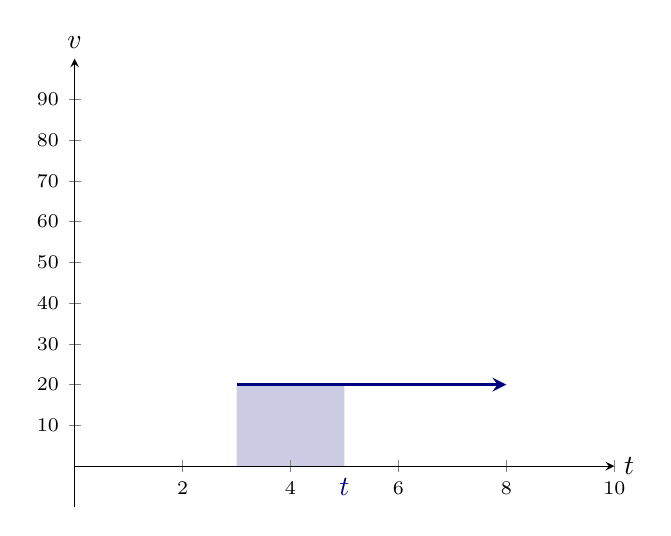
\begin{tikzpicture}
  \begin{axis}[
            domain=0:10, ymax=100, xmax=10, ymin=-10, xmin=0,
            axis lines =center, xlabel=$t$, ylabel=$v$, 
            ytick={0, 10, 20, 30, 40, 50, 60, 70, 80, 90},
            xtick={0, 2, 4, 6, 8, 10},
            ticklabel style={font=\scriptsize},
            every axis y label/.style={at=(current axis.above origin),anchor=south},
            every axis x label/.style={at=(current axis.right of origin),anchor=west},
            axis on top
          ]
          

			\addplot [draw=penColor, very thick, smooth, domain=(3:8),->] {20};
			%\addplot[color=penColor,fill=penColor,only marks,mark=*] coordinates{(0,50)};



			\addplot [name path=A,domain=3:5,draw=none] {20};   
			\addplot [name path=B,domain=3:5,draw=none] {0};
			\addplot [fillp] fill between[of=A and B];

			\draw[penColor,thick] (30,10) -- (30,30);
			\draw[penColor,thick] (50,10) -- (50,30);

			\node at (axis cs:5,-5) [penColor] {$t$};



  \end{axis}
\end{tikzpicture}
\end{image}
The area is still $length \cdot height$.



\begin{itemize}
\item length = $t - 3$
\item height = $v(t) = 20$
	\end{itemize}




\[
Area = 20(t-3)
\]



The area under the velocity graph represents the accumulated distance travelled.






\[
D(t) = 20(t-3) \, \text{ for }  \, t \geq 3
\]








\begin{image}
\begin{tikzpicture}
  \begin{axis}[
            domain=0:10, ymax=100, xmax=10, ymin=-10, xmin=0,
            axis lines =center, xlabel=$t$, ylabel=$D$, 
            ytick={0, 10, 20, 30, 40, 50, 60, 70, 80, 90},
            xtick={0, 2, 4, 6, 8, 10},
            ticklabel style={font=\scriptsize},
            every axis y label/.style={at=(current axis.above origin),anchor=south},
            every axis x label/.style={at=(current axis.right of origin),anchor=west},
            axis on top
          ]
          

			\addplot [draw=penColor, very thick, smooth, domain=(3:7),->] {20*(x-3)};
			%\addplot[color=penColor,fill=penColor,only marks,mark=*] coordinates{(0,50)};









  \end{axis}
\end{tikzpicture}
\end{image}

The region under the graph of $D(t)$ now forms a triangle.














\begin{image}
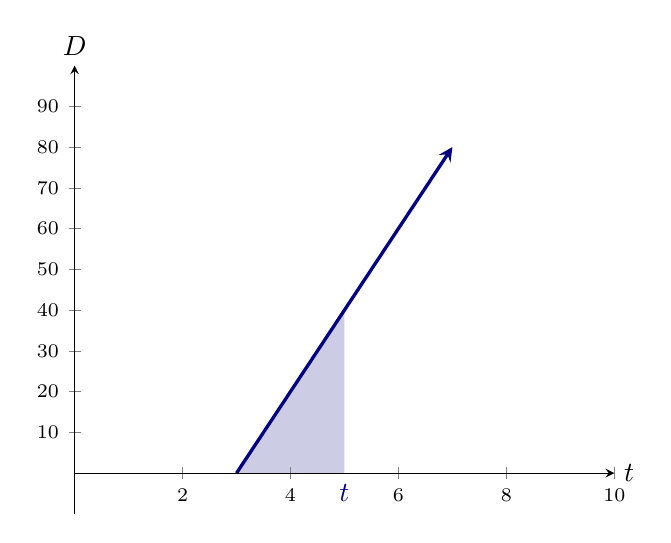
\begin{tikzpicture}
  \begin{axis}[
            domain=0:10, ymax=100, xmax=10, ymin=-10, xmin=0,
            axis lines =center, xlabel=$t$, ylabel=$D$, 
            ytick={0, 10, 20, 30, 40, 50, 60, 70, 80, 90},
            xtick={0, 2, 4, 6, 8, 10},
            ticklabel style={font=\scriptsize},
            every axis y label/.style={at=(current axis.above origin),anchor=south},
            every axis x label/.style={at=(current axis.right of origin),anchor=west},
            axis on top
          ]
          

			\addplot [draw=penColor, very thick, smooth, domain=(3:7),->] {20*(x-3)};
			%\addplot[color=penColor,fill=penColor,only marks,mark=*] coordinates{(0,50)};




			\addplot [name path=A,domain=3:5,draw=none] {20*(x-3)};   
			\addplot [name path=B,domain=3:5,draw=none] {0};
			\addplot [fillp] fill between[of=A and B];


			\draw[penColor,thick] (50,10) -- (50,50);

			\node at (axis cs:5,-5) [penColor] {$t$};




  \end{axis}
\end{tikzpicture}
\end{image}





The area under the graph of $D(t)$ now forms a triangle, with base $t-3$ and height $D(t) = 20(t-3)$.



We now have a formula for the accumulated area under the graph of $D(t) = 20(t-3)$.


\[
A(t) = \frac{1}{2} (t-3) \cdot 20(t-3) = 10 (t-3)^2   \, \text{ for }  \, t \geq 3
\]








\begin{image}
\begin{tikzpicture}
  \begin{axis}[
            domain=0:10, ymax=100, xmax=10, ymin=-10, xmin=0,
            axis lines =center, xlabel=$t$, ylabel=$A$, 
            ytick={0, 10, 20, 30, 40, 50, 60, 70, 80, 90},
            xtick={0, 2, 4, 6, 8, 10},
            ticklabel style={font=\scriptsize},
            every axis y label/.style={at=(current axis.above origin),anchor=south},
            every axis x label/.style={at=(current axis.right of origin),anchor=west},
            axis on top
          ]
          

			\addplot [draw=penColor, very thick, smooth, domain=(3:5),->] {20*(x-3)^2};
			%\addplot[color=penColor,fill=penColor,only marks,mark=*] coordinates{(0,50)};






  \end{axis}
\end{tikzpicture}
\end{image}

Rate of change and accumulation are two sides of the same coin.  They tell the same story forwards and backwards.



There is a reverse relationship between rate of change and accumulation.


$\blacktriangleright$ The constant function $20$ gives the rate of change of the linear function $20(t-3)$.


$\blacktriangleright$ The linear function $20(t-3)$ is the accumulation function of the constant function $20$.




We have now seen that \\

$\blacktriangleright$ The quadratic function $10(t-3)^2$ is the accumulation function of the linear function $20(t-3)$. \\





\begin{claim}


The linear function $20(t-3)$ gives the rate of change of the quadratic function $10(t-3)^2$.



\begin{idea}


Let $A(t) = 10 (t-3)^2$


The rate of change of $A(t)$ over the interval $(3, t)$ is given by




\[
\frac{\Delta A}{\Delta t} = \frac{A(t) - A(3)}{t-3} = \frac{10 (t-3)^2}{t-3} = 10(t-3)
\]


Not Quite!  But, close.  It is off by a factor of $2$.  

\end{idea}


Hmmm!

\end{claim}














The story is off a little bit. We need a new perspective on rate of change.  A slight adjustment will align rate of change and accumulation as different directions of the same story. \\

Stay tuned!










\begin{center}
\textbf{\textcolor{green!50!black}{ooooo-=-=-=-ooOoo-=-=-=-ooooo}} \\

more examples can be found by following this link\\ \link[More Examples of Linear Functions]{https://ximera.osu.edu/csccmathematics/precalculus1/precalculus1/linearFunctions/examples/exampleList}

\end{center}






\end{document}
